\setcounter{rownumber}{0}
\singlespacing
\chapter{Brillouin-Induced Raman Modes and Device Exploration}
\label{ch:Raman}
\acresetall

\doublespacing

%%%%%%%%%%%%%%%%%%%%%%%%%%%%%%%%%%%%%%%%%%%%%%%%%%%%%%%%%%%%%%%%%%%%

\section{Introduction}
\label{sec:Raman:Introduction}

motivation, context, Brillouin->Raman transition

%--------------------------------------------------------------------%

\section{Brillouin-Induced Raman Modes}
\label{sec:Raman:Brillouin-Induced}

\subsection{Brillouin-Raman Transition}
\label{subsec:Raman:Brillouin-RamanTransition}

autointerfering traveling-wave phonons

\begin{figure}[t]
  \centering
  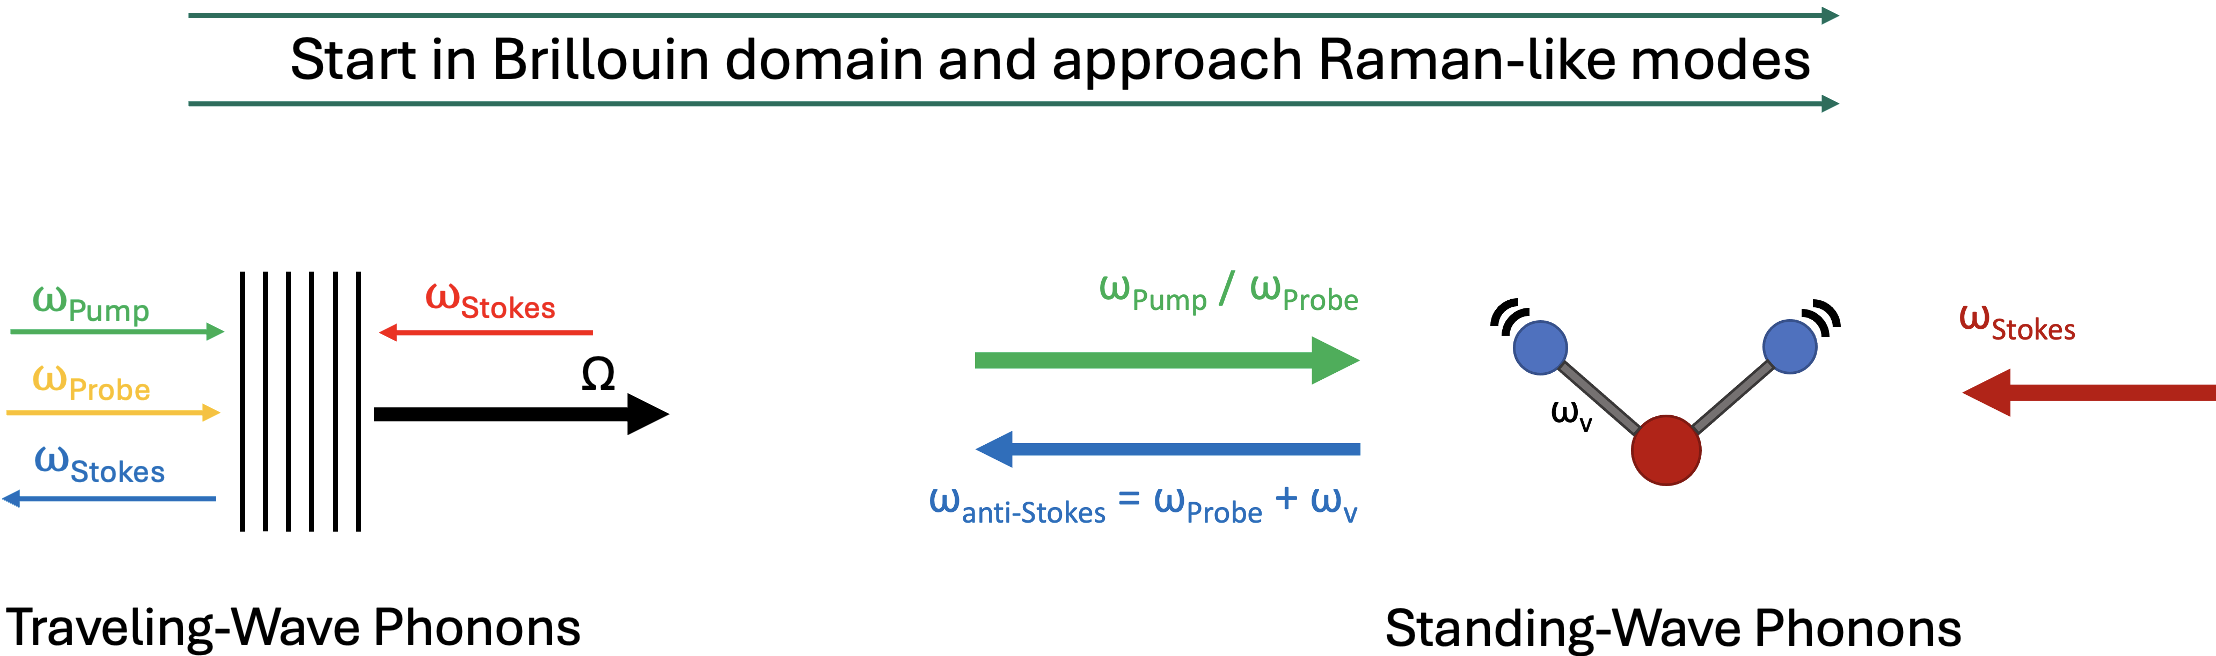
\includegraphics[width=\textwidth]{figs/4-Raman/ExploreBrillouinRamanTransition.png}
  \caption{Transition from Brillouin domain to Raman-like modes.}
  \label{fig:BrillouinRamanTransition}
\end{figure}

\begin{figure}[t]
  \centering
  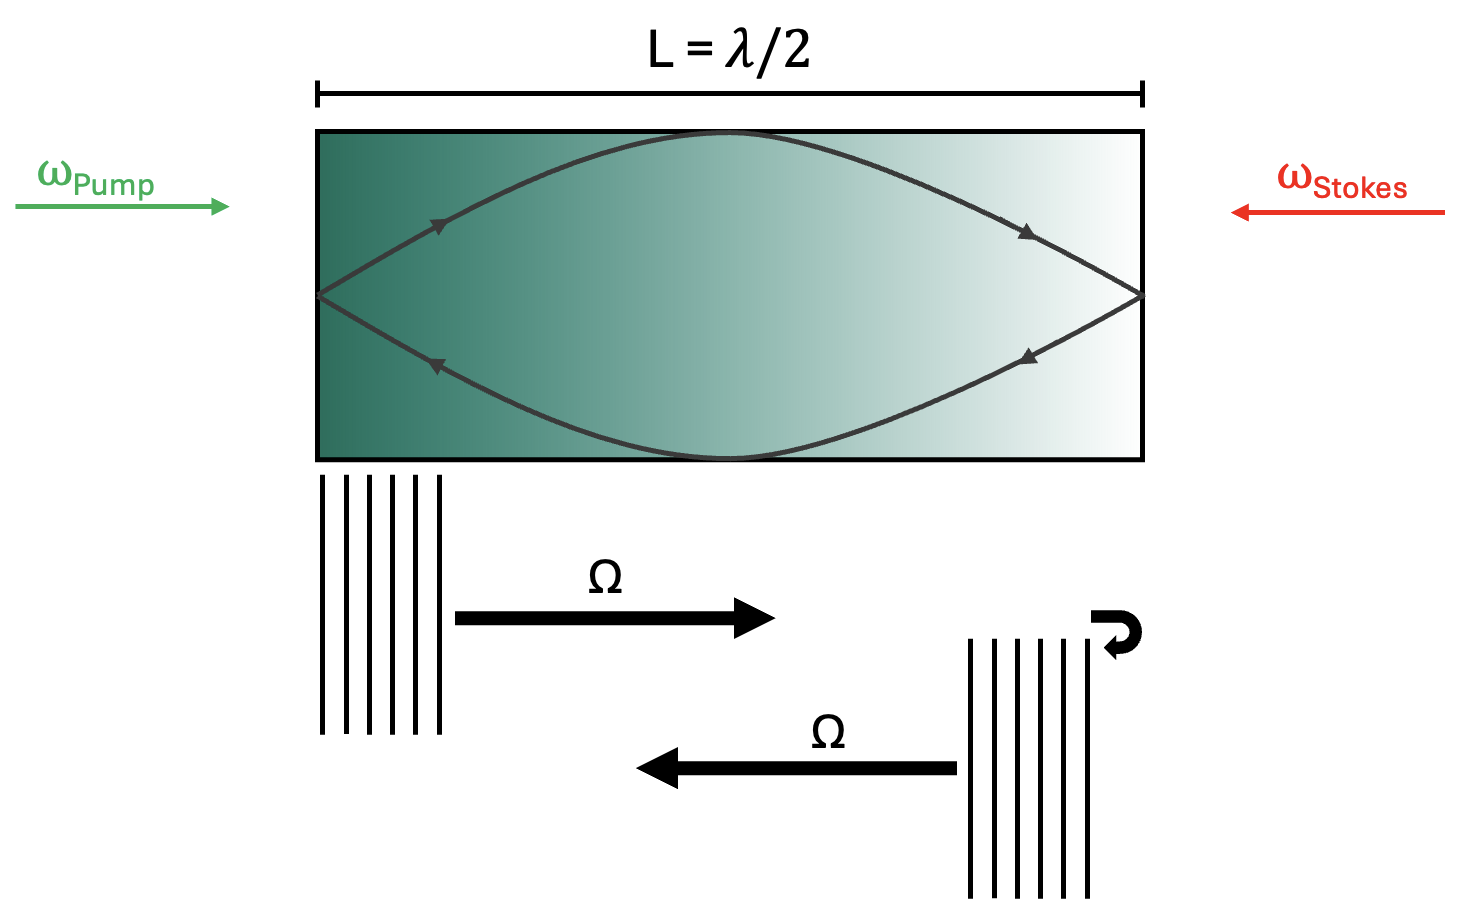
\includegraphics[width=.85\textwidth]{figs/4-Raman/GeometryDeterminesFundamentalFreq.png}
  \caption{Geometry determines fundamental frequency.}
  \label{fig:GeometryDeterminesFundamentalFreq}
\end{figure}

\begin{figure}[t]
  \centering
  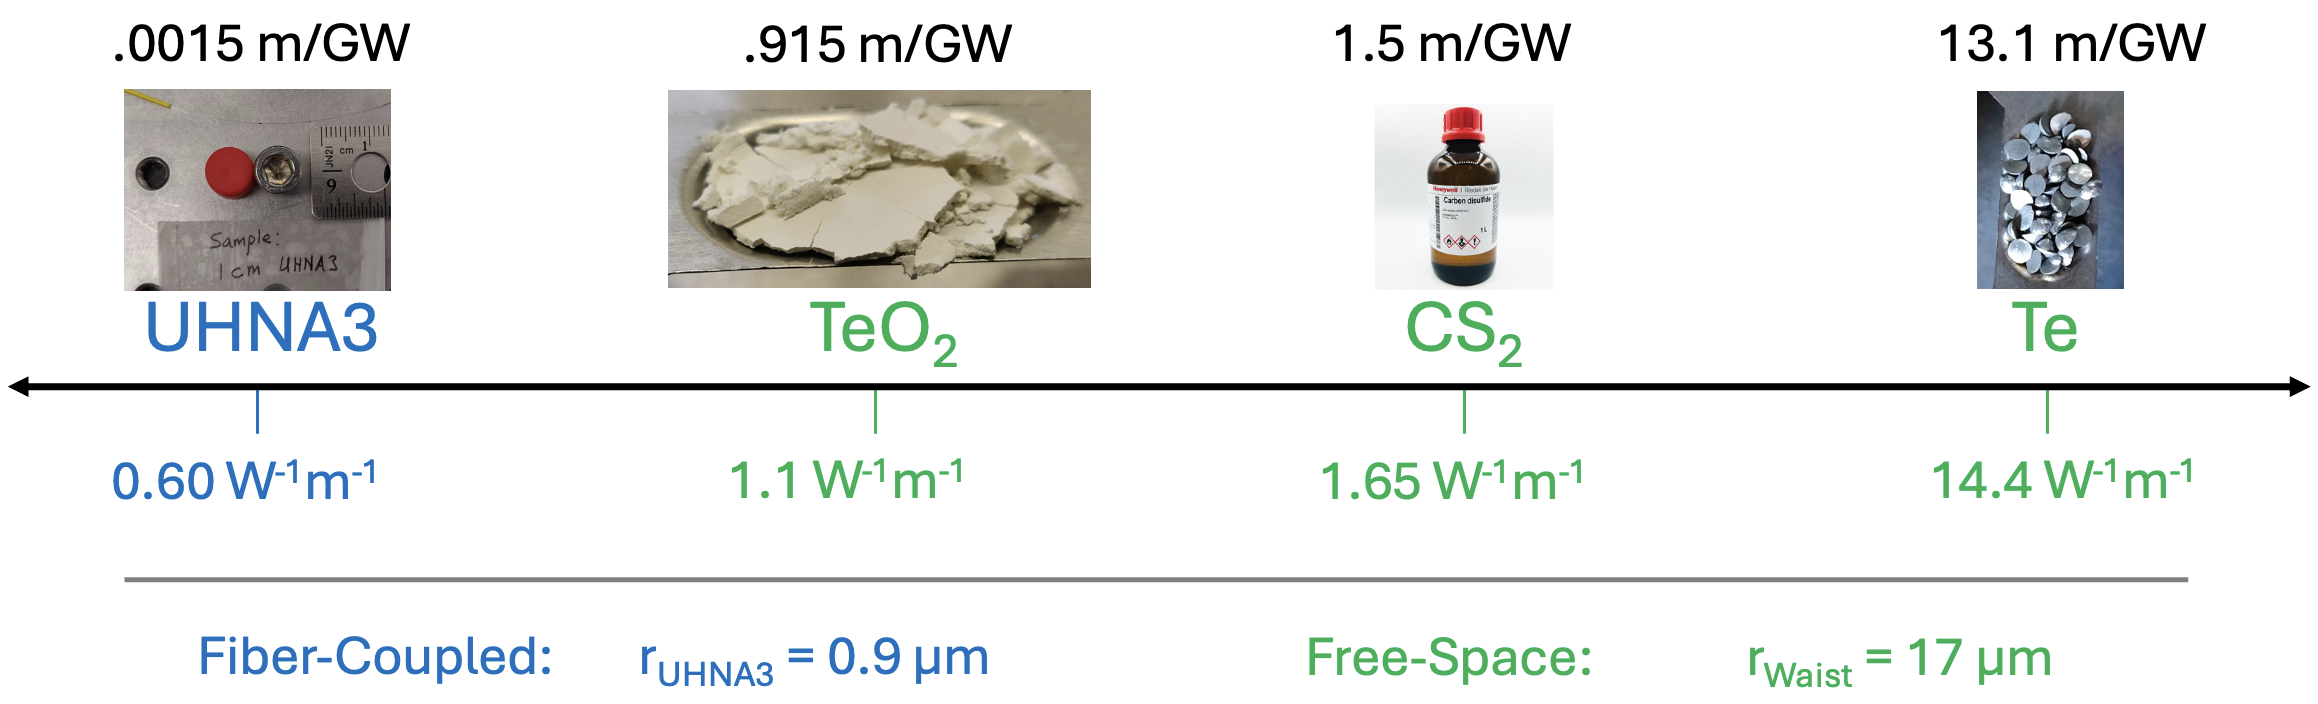
\includegraphics[width=\textwidth]{figs/4-Raman/GainOfRelevantMaterials.png}
  \caption{Gain of relevant materials.}
  \label{fig:GainOfRelevantMaterials}
\end{figure}

\subsection{Acoustic Impedance and Reflection}
\label{subsec:Raman:AcousticImpedanceAndReflection}

\begin{figure}[t]
  \centering
  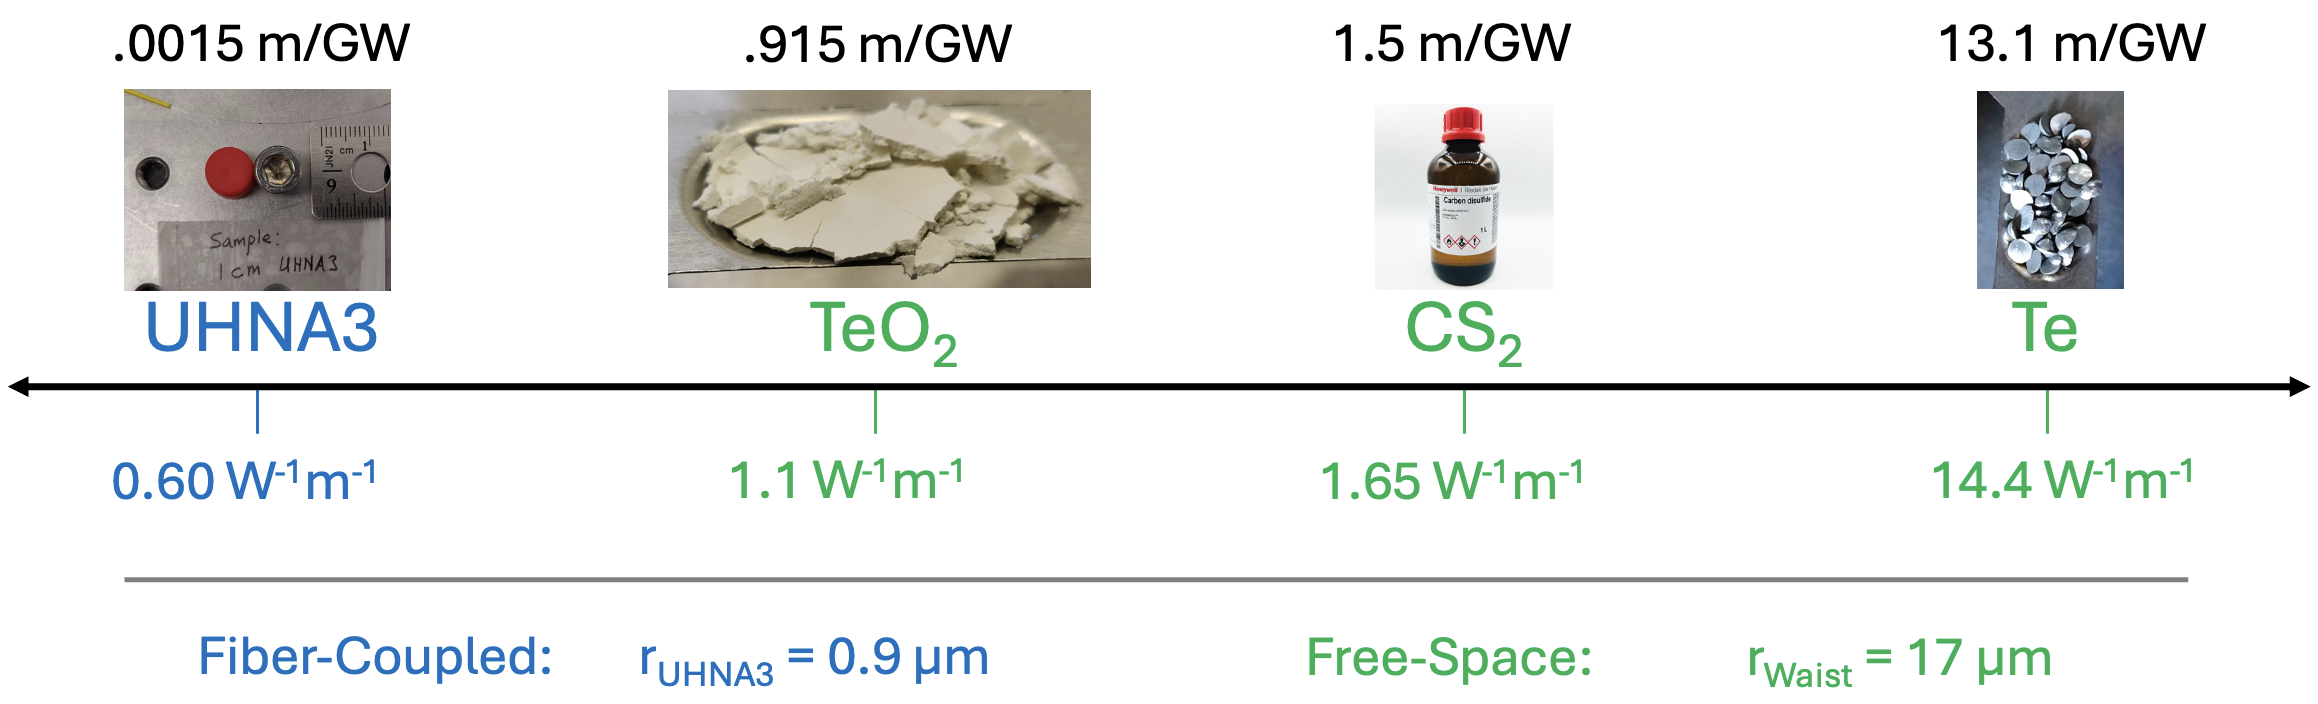
\includegraphics[width=\textwidth]{figs/4-Raman/GainOfRelevantMaterials.png}
  \caption{Gain of relevant materials.}
  \label{fig:GainOfRelevantMaterials}
\end{figure}

\subsection{Phonon Lifetime}
\label{subsec:Raman:PhononLifetime}

phonon mean travel distance

%--------------------------------------------------------------------%

\section{Target Platform Evolution and Collaborative Fabrication}
\label{sec:Raman:TargetPlatforms}

\subsection{Germanium-Doped Optical Fiber}
\label{subsec:Raman:Target:UHNA3}

1cm -> 1mm

\subsection{Free-Space Optics with Liquid Carbon Disulfide}
\label{subsec:Raman:Target:CS2Vial}

Free space with vial

\subsection{Tellurium Dioxide Thin Film}
\label{subsec:Raman:Target:TeO2}

Gibbs collab -> acoustic dissipation into substrate (dissolve, sheet music)

\subsection{Tellurium Thin Film}
\label{subsec:Raman:Target:Te}

Gibbs collab -> CINT collab -> oxidizes to TeO2

\subsection{Carbon Disulfide Micrometer Cell}
\label{subsec:Raman:Target:CS2Cells}

cells -> 1 W amp, bubble test

\subsection{Suspended Silica Rib Waveguide}
\label{subsec:Raman:Target:Waveguide}

BYU collab -> initial test took 9 months to learn and measure

\subsection{Elastically-Suspended Photonic-Phononic Waveguide}
\label{subsec:Raman:Target:WigglyWaveguide}

BYU collab - proof of fabrication: holes and trampoline

%--------------------------------------------------------------------%

\section{Results}
\label{sec:Raman:Results}

UHNA3 - 1cm, 1mm
CS2 vial - 4mm, 2mm
TeO2 films - 1um, 500nm
CS2 - 1mm, 100um, (10um not quite)
chip waveguide - chip/nochip, holes

\begin{figure}[t]
  \centering
  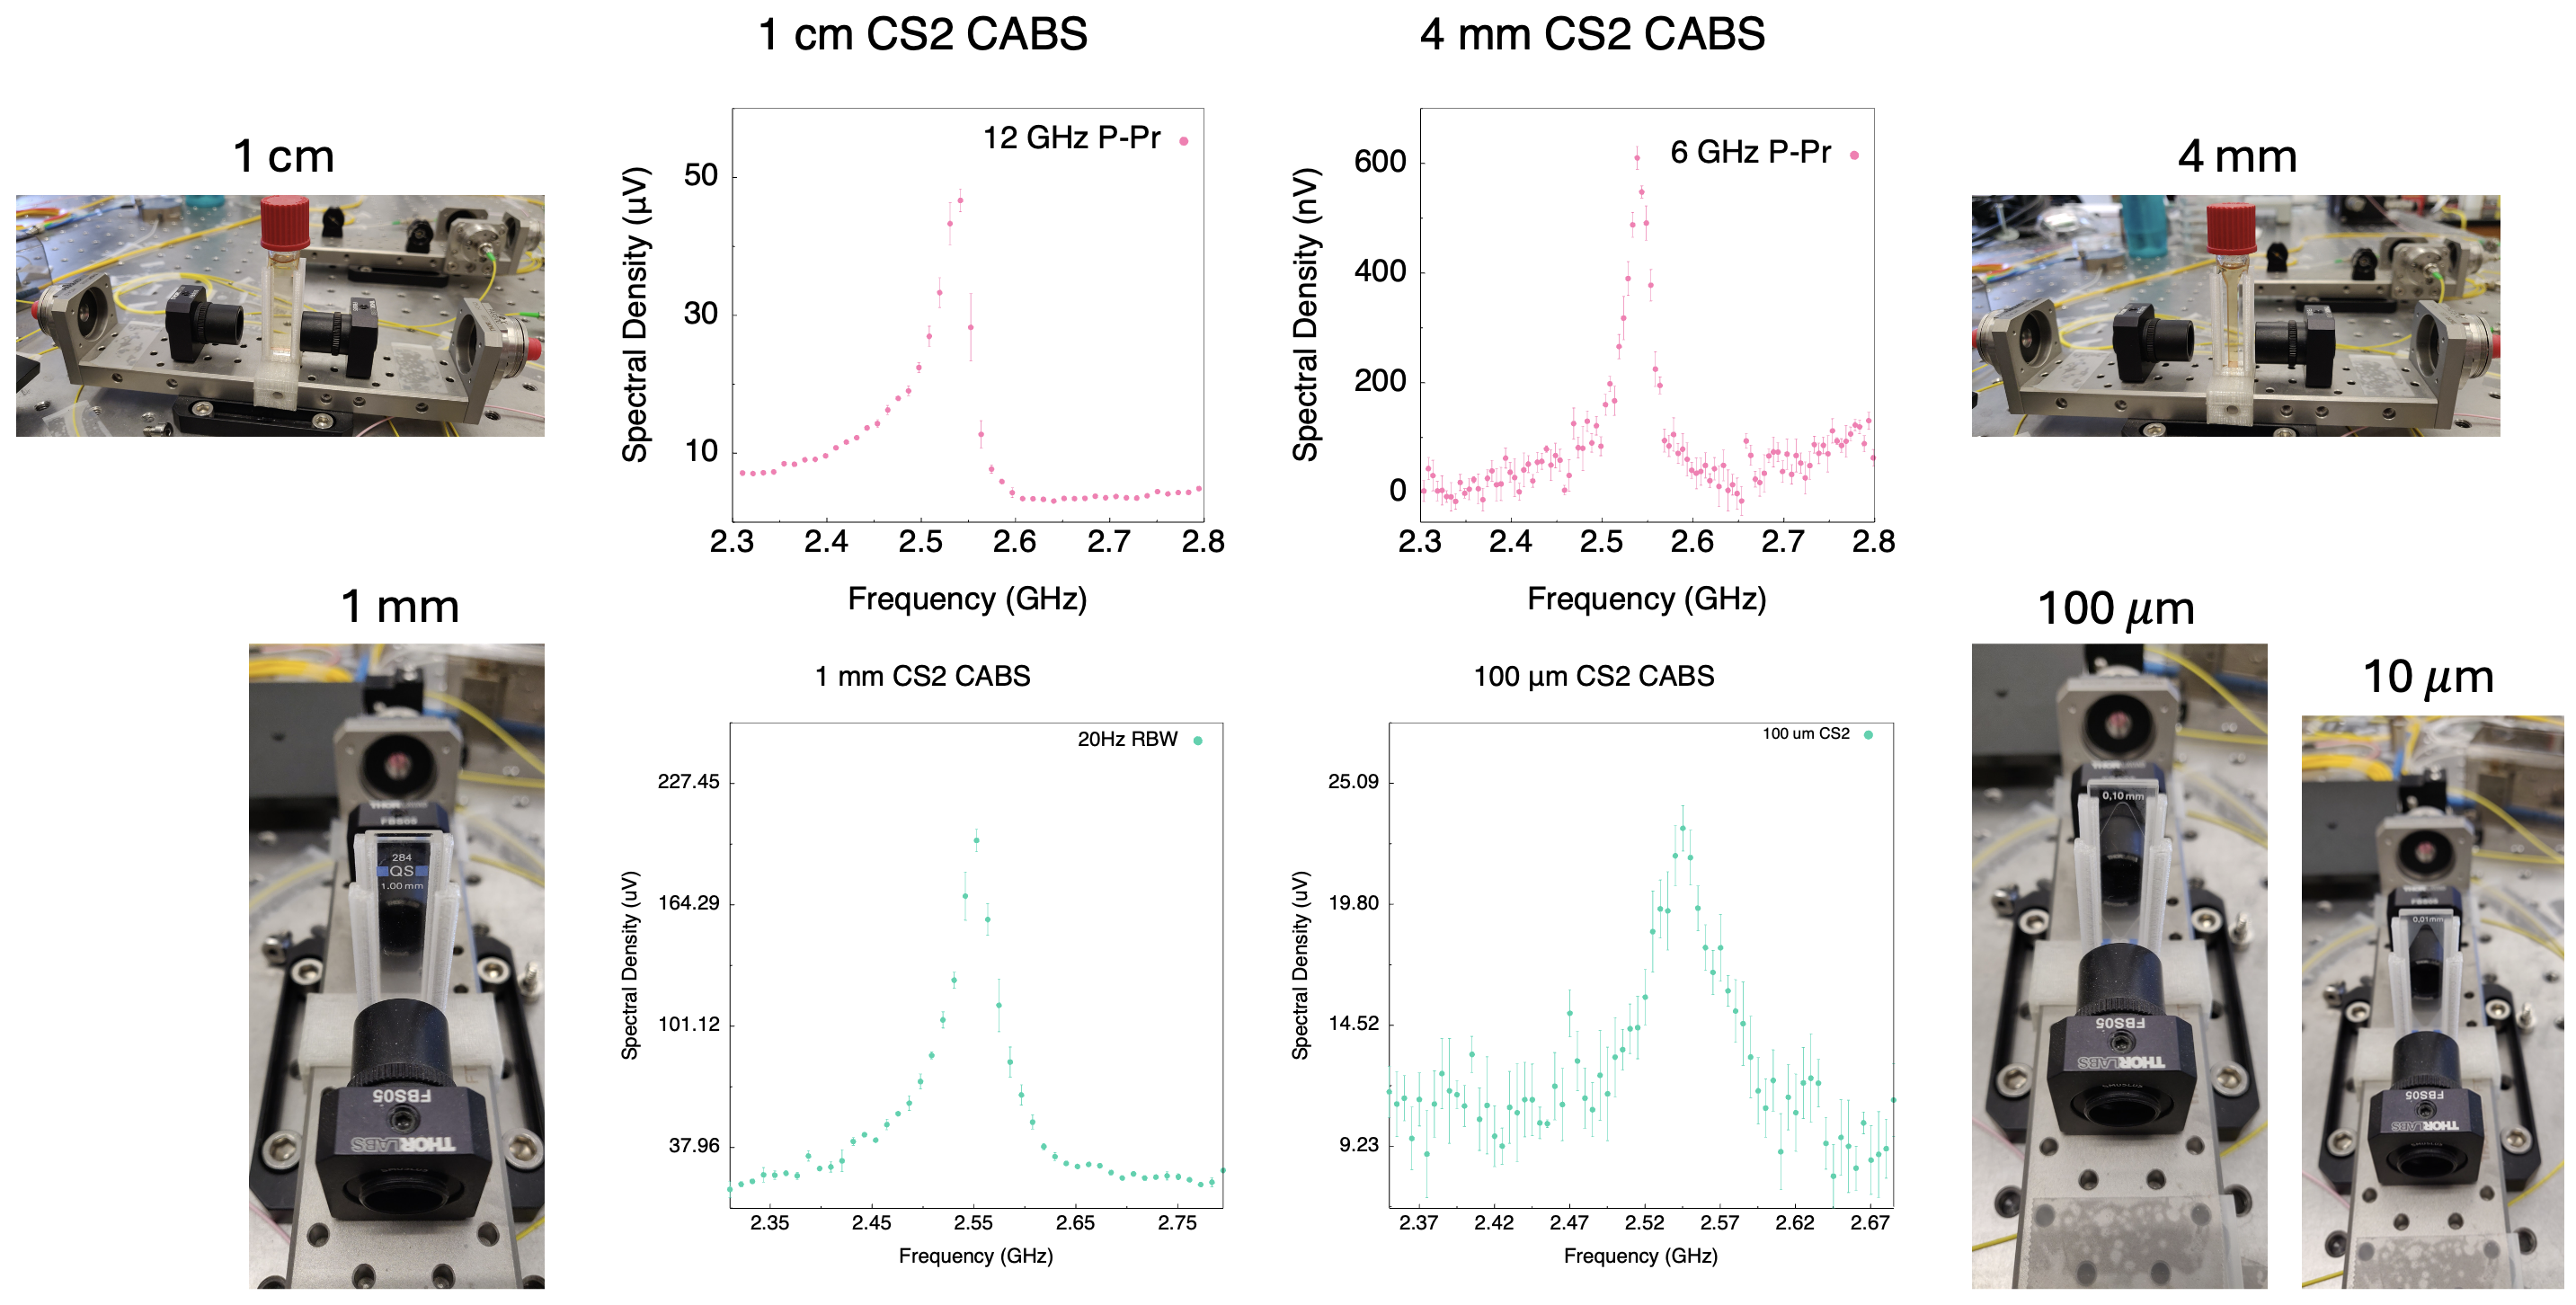
\includegraphics[width=\textwidth]{figs/4-Raman/StartBigApproachSmall.png}
  \caption{Start big, approach small.}
  \label{fig:StartBigApproachSmall}
\end{figure}

\begin{figure}[t]
  \centering
  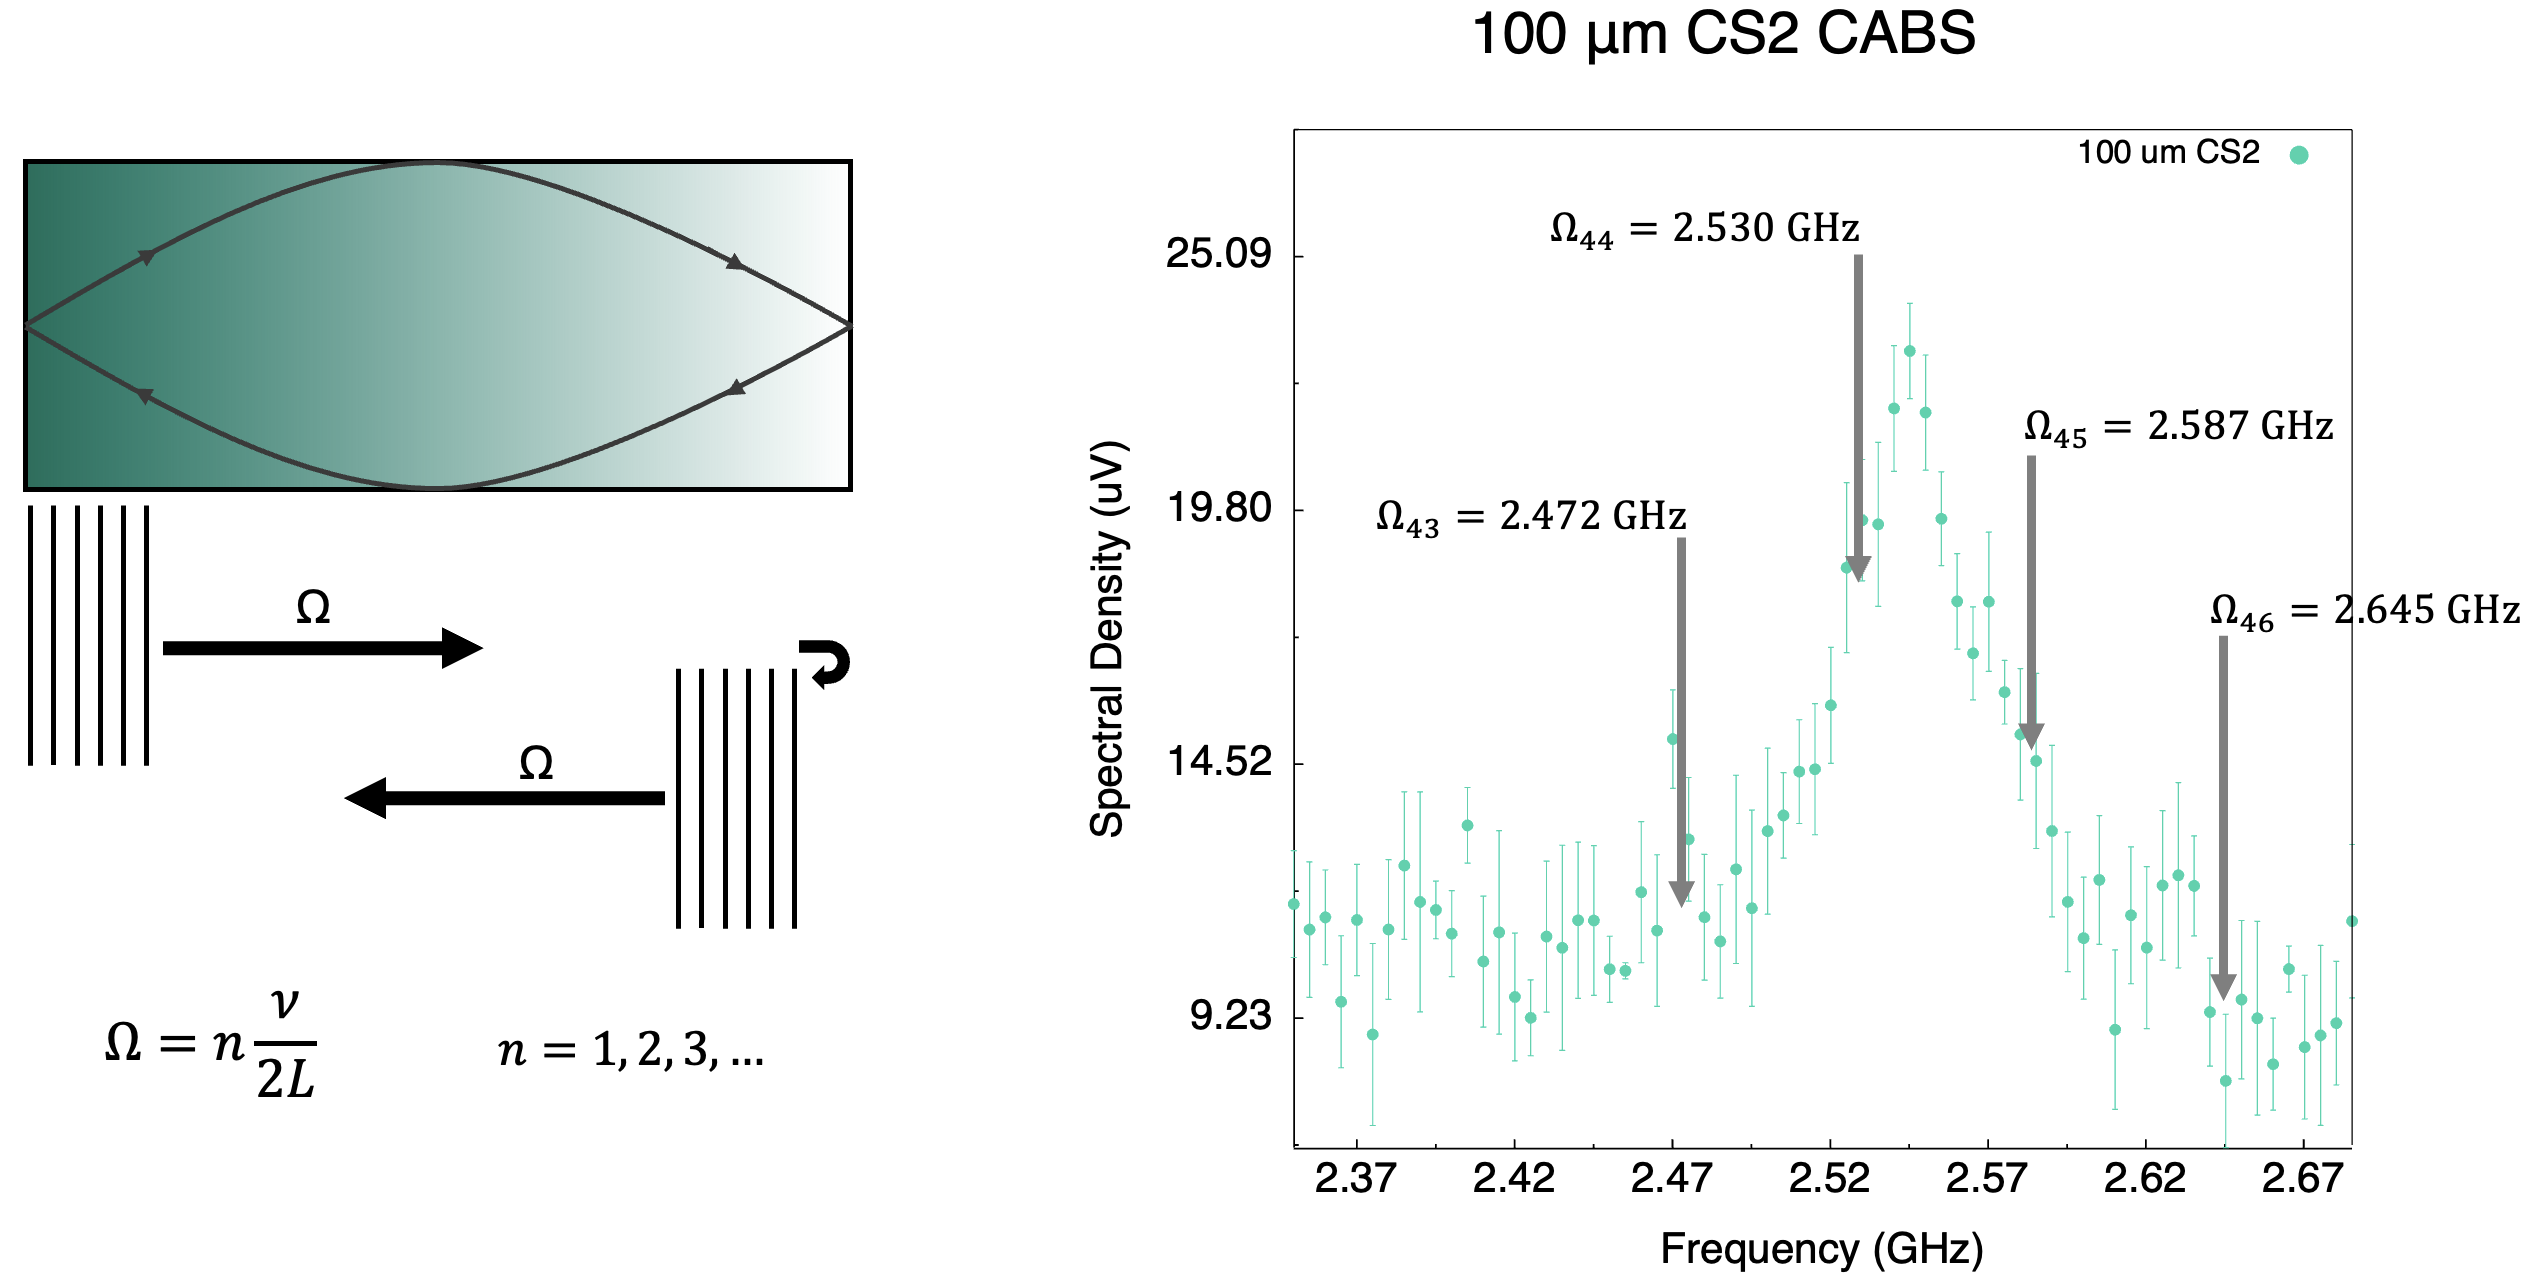
\includegraphics[width=\textwidth]{figs/4-Raman/HowWouldRamanModesAppear.png}
  \caption{How would Raman modes appear.}
  \label{fig:HowWouldRamanModesAppear}
\end{figure}

%--------------------------------------------------------------------%

\section{Discussion}
\label{sec:Raman:Discussion}

\subsection{Pathways to Brillouin-Induced Raman Modes}
\label{subsec:Raman:Pathways}
Ideal platforms by category
  waveguide - long TeO2 rib, evenly spaced square holes
  TeO2 thin film/crystal - dissolve only small area of substrate for beam spot
  CS2 cell

\subsection{Conclusion}
\label{subsec:Raman:Conclusion}


\clearpage
\thispagestyle{empty}
\null
\newpage
